\documentclass[10pt,letterpaper,unboxed,cm]{article}
\usepackage{tgtermes} % times font
\usepackage{setspace}
%\doublespacing

\usepackage[margin=1in]{geometry}
\usepackage{graphicx}
\usepackage{amsmath}
\usepackage{amssymb}
\usepackage{xcolor}
\usepackage[export]{adjustbox}
\usepackage[linesnumbered,lined]{algorithm2e}
\usepackage{enumerate}
\usepackage[symbol]{footmisc}
\usepackage{textcomp}
\usepackage{dirtytalk}

\newcommand{\st}{~\mid~}
\newcommand{\ind}{$~~~$}
\newcommand{\todo}{\color{red} TODO: \color{black}}

\graphicspath{{images/}}

\renewcommand{\thefootnote}{\fnsymbol{footnote}}

\newcommand\blfootnote[1]{%
  \begingroup
  \renewcommand\thefootnote{}\footnote{#1}%
  \addtocounter{footnote}{-1}%
  \endgroup
}

\interfootnotelinepenalty=10000

\title{OpenOBD}

\date{June 10th, 2020}

\author{Cody Emrick\\A14740612 \and Christopher Madrigal\\A15702734}

\begin{document}

\maketitle

%\blfootnote{* From Special Collections}

\renewcommand*{\thefootnote}{\arabic{footnote}}

\tableofcontents
\newpage

\section{Abstract}

Vehicles seem to perpetually exist in a bygone era. By the time new cars adopt a technology, whether it be radio, CD players, or navigation systems, there's a very good chance that a similar feature has been available elsewhere for years beforehand. And when you want to upgrade, you will need to buy a new car to do so. Worst of all, you'll likely end up with a proprietary, custom solution with limited features. Shopping for a car based on the quality of the infotainment system is impractical, and even high-end cars are subject to this problem. Likewise, home mechanics that want access to diagnostic data will need to purchase a specialized, manufacturer-specific device just to read data. All vehicles since the mid-1990's come equipped with a standardized onboard diagnostic (OBD) system, but manufacturers and professional mechanics have done everything they can to lock consumers out of these vital systems. Our project proposes to break their monopoly on your car's data by allowing users and developers a safe, easy way to access and utilize data to enhance your vehicle's functionality and allow for modular upgrades.

\section{Introduction}

\subsection{The Problem}

Fundamentally, the core problem here is that most vehicles do not operate on a standard platform. Even similar models by the same manufacturer might only have a few parts in common, and even when a manufacturer creates a standardized platform, it's more for their benefit than the customer's and eventually they will do a refresh that will break compatibility. This forces aftermarket parts to be built around a specific make and model, perhaps with some flexibility based on the year or platform. Regardless, this has led to a quagmire of compatibility issues. For an aftermarket part manufacturer, there is little incentive to release an upgrade for a car nobody is buying new anymore. 

We can further sub-divide this problem into two classes: physical and electron. For example, if you want to buy a new radio for your car, you need to find one that both fits physically into your dashboard and also will connect to your car's audio system. On modern cars, your \say{infotainment} system may also contain many of the controls for your vehicle, or also display select diagnostic information, which means it must interface with whatever wiring and information specification the manufacturer provides. Our goal will be to tackle the latter issue, and we believe that, free of a requirement to match proprietary data connections, it will be easier to adapt a generic product to fit physically in a variety of vehicles. Even on modern vehicles with an Apple CarPlay or Android Auto are often difficult to upgrade and will not have access to a full range of information, although they are a step in the right direction.

\subsection{The Goal}

We believe that someone looking to upgrade their vehicle should simply be able to go online or to a store, browse products that solve a problem they have, and then be able to use this in their car. They should not have to be locked-in to a given vendor or system, nor should they have to fear that they will lose access to their data or control of their car. As vehicles trend increasingly towards being \say{smart}, \say{Internet of Things} objects, the issues inherent in the modern smart-device ecosystem creep in to a traditionally very stable platform, and nobody should have to worry about their car being disabled or damaged remotely via exposure to a broader network. 

Additionally, as creators, we want more freedom to get data from our cars and to experiment with solutions to the problems with have. This is the basis of innovation, and currently any individual hoping to create a new product will have to navigate a technical minefield just to develop a one-off product for their own vehicle. A single man working alone ought to be able to create a solution and share this with others in whatever way they see fit. This is a fundamental aspect of \say{hacker culture}, and by lowering the bar to creating novel solutions we hope to spur innovation in this market.

\subsection{Our Solution}

However, all vehicles since the mid-1990's come equipped with the OBD-II specification for onboard diagnostics. This federally-mandated system provides a common interface for storing and accessing data relevant to your car's performance. Some manufacturers choose to build on top of this system to expand functionality.

With the above problems and goals in mind, we created the following guidelines for our device:

\begin{description}

\item [It Must Be Open:] In order for users to build on our work and audit its security, the platform must be open. A closed platform just adds one more inflexible, untrustworthy option.

\item [It Must Be Secure:] We want to authenticate communications between the user and their vehicle. While secrecy of the data is important, ensuring that requests come from and responses are returned to the owner of the vehicle and their authorized devices only is absolutely the most important thing. If the platform is insecure, it could leak private information about the user to malicious third-parties, or in a worst-case scenario, cause damage to their vehicle.

\item [It Must Be Safe:] The platform itself should reliably interface with vehicles without causing any harm. A developer should not be concerned that a bad write will brick their car's diagnostic computer. They must trust it to intercept and sanitize inputs to prevent mistaken or malicious commands.

\item [It Must Be Expandable:] The core set of OBD-II functions is standard across all vehicles, but we must allow for users to support additional functionality their manufacturer may provide. Additionally, users who want to write their own software or make their own hardware should be able to easily prototype on top of our platform.

With these goals in mind, we were able to take a common-sense approach to the design of our device, dubbed OpenOBD, which would allow us to interface easily with other devices while providing reliable service.

\end{description}

\section{Technical Material}

\subsection{Prior Work}

\todo Examination of other products on the market and which of the above points they fail on.

\subsection{Design}

\begin{center}
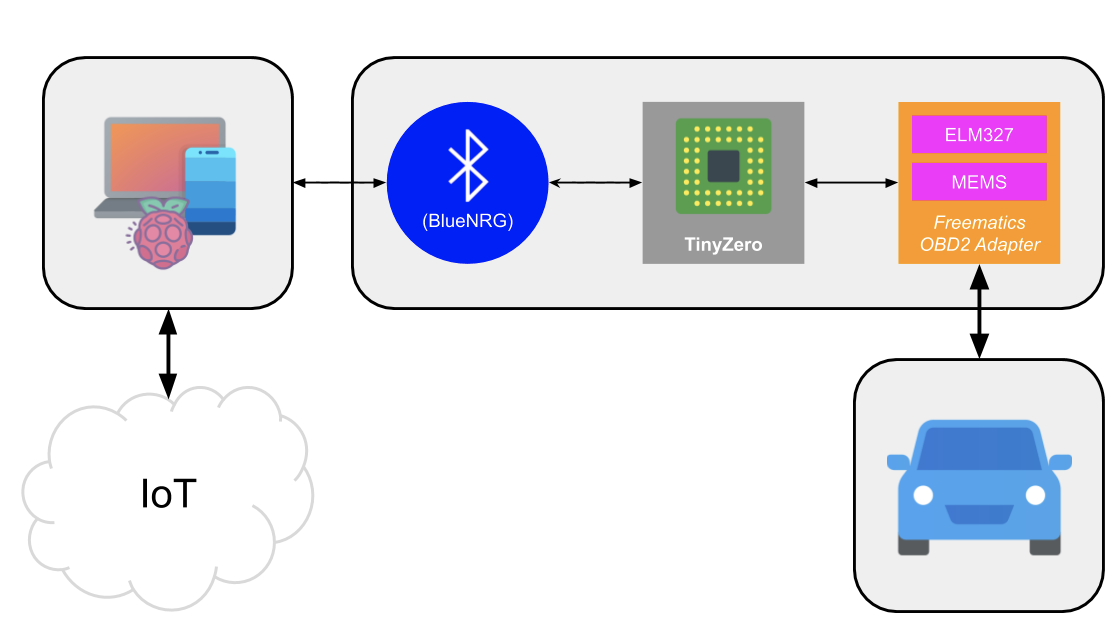
\includegraphics[width=0.7\linewidth]{pathway.png}
\end{center}

\todo High-level description of system.

\subsection{Platform}

\todo Why we chose TinyZero and ELM.

\section{Milestones}

\begin{description}

\item [Read Data:] Physically read data from a device.
\item [Write Data:] Physically write data to the device.
\item [Expose Data:] Expose the data via an API
\item [Example Application:] Create a simple app that showcases how to use the API. Can also be used for debugging purposes.
\item [Encrypt Data:] Take this datapath and add user authentication.
\item [Allow Modifying Vehicle State:] Expose safe writes to the vehicle.
\item [Additional Sensors:] Add additional sensors to the device which cannot be found on many cars, such as GPS, accelerometer, etc.

\end{description}

\subsection{Read Data}

\todo Explain how we wrote to conform to provided ELM driver and how we didn't get the actual connector delivered.

\subsection{Write Data}

\todo Explain how we wrote to conform to provided ELM driver and how we didn't get the actual connector delivered.

\subsection{Expose Data}

\todo Explain the API and JSON implementation.

\subsection{Encrypt Data}

\todo done via RSA encryption. Explain how this is asymmetric. Explain how this  verifies the user is allowed to make a request, and while it does help protect the data much of that lies within the Bluetooth spec. So there's two layers of encryption here.

\subsection{Allow Modifying Vehicle State}

\todo Dropped because the writes aren't very important and sanitizing inputs requires thought, so it got backburnered.

\subsection{Additional Sensors}

\todo Say we added a GPS and some storage to facilitate GPS and prepare for adding SIM card support.

\section{Conclusion}

\section{References}


%\footnote{\label{klooster}\textit{Revolutions in the Atlantic World}, Wim Klooster, 2018, New York Press}

\end{document}

